\section{Basic and Dynamic Smagorinsky Code adjustment}
In addition to expanding out the index notation for the enstrophy
production, I have also been working on adjusting the pseudo spectral code
to allow the user to switch between the basic and dynamic Smagorinsky.
After adjusting the code various runs were conducted to determine if it was
possible to increase the stability by turning on the dynamic Smagorinsky
after the initial conditions have stabilized. The results from these
simulations conclude that there is no stability gained by postponing to
turn on the dynamic Smagorinsky model. 

\subsection{Results}
The results presented below are for a simulation that correspond to a 
total subgrid stress $\tau_{ij}$ calculated as, 
\begin{equation}
    \tau_{ij} = (1-C_{DS})\tau_{ij}^{BS} + C_{DS}\tau_{ij}^{DS}
\end{equation}
where $\tau_{ij}^{BS}$ is the basic Smagorinsky subgrid stress, and
$C_{DS}$ and $\tau_{ij}^{DS}$ are the dynamic Smagorinsky coefficient and
subgrid stress respectively. Furthermore, the dynamic coefficient was defined
as an ``on/off'' switch, namely,
\begin{equation}
    C_{DS} \equiv          
    \begin{cases}
        0.0     \text{ for $0 \leq t^{*} < 50 $}            \\
        0.60    \text{ for $50 \leq t^{*} < 100 $}          \\
        0.0     \text{ for $100 \leq t^{*} \leq 150 $}      \\
        0.60    \text{ for $150 \leq t^{*} \leq 200 $}      \\
    \end{cases}
\end{equation}
where $t^{*}$ is the simulation time. Figure~\ref{fig:bs-ds-smagorinsky}
displays the results for the average kinetic energy versus time, where it
is evident that delaying turning on the dynamic Smagorinsky does not
improve the stability of the simulation.

\begin{figure}[H]
    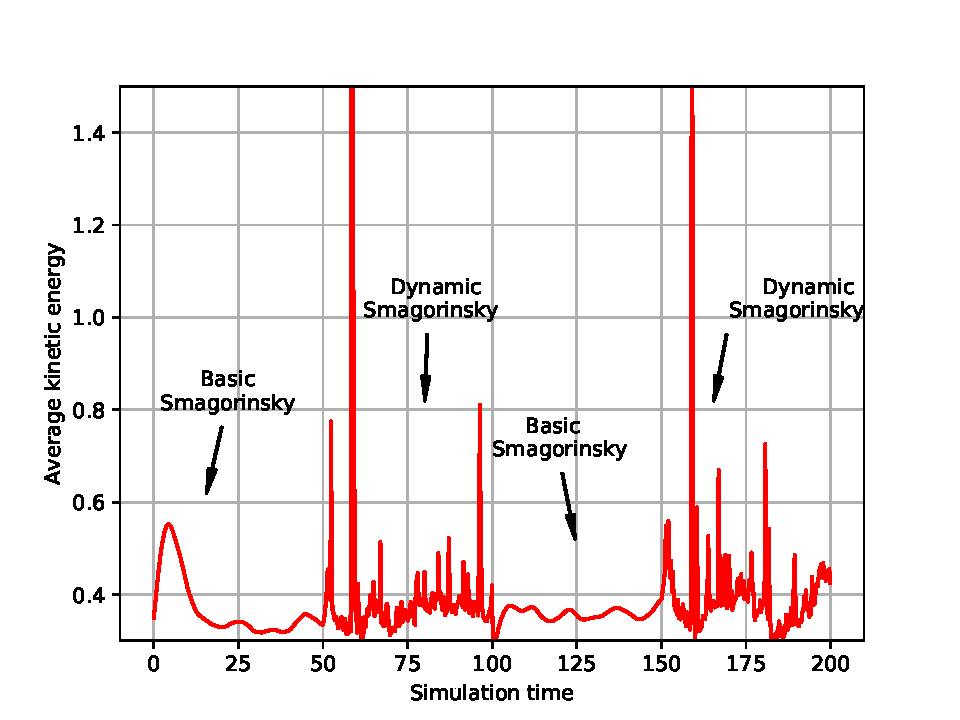
\includegraphics[height=0.4\textheight]{media/ke-avg-DS-00-60}
    \caption{Average kinetic energy versus simulation time}
    \label{fig:bs-ds-smagorinsky}
\end{figure}

Therefore, we can now run simulations with the ability to switch between
basic and dynamic Smagorinsky, however this does nothing in terms of
stability. 
